%--------------------
% Packages
% -------------------
\documentclass[10pt,a4paper]{article}

\usepackage{iftex} % <-- Add this to check the compiler

% Only load microtype if compiling with pdfLaTeX
\ifPDFTeX
  \usepackage[protrusion=true,expansion=true]{microtype}
\fi

\usepackage{fontspec}
\usepackage{polyglossia}
\setmainlanguage{polish}
\setmainfont{Verdana} % Set Verdana as the main font

\usepackage{ragged2e}

\usepackage{graphicx} % No [pdftex] option here! XeLaTeX will auto-detect
\usepackage[
  colorlinks=true,
  linkcolor=black,
  urlcolor=black,
  citecolor=black,
  pdfborder={0 0 0}
]{hyperref} % Proper hyperref setup for xelatex

\usepackage{calc}
\usepackage{enumitem}

\frenchspacing
\linespread{1.15}

\usepackage[a4paper, lmargin=3.5cm, rmargin=2.5cm, tmargin=2.5cm, bmargin=2.5cm]{geometry}

\usepackage[all]{nowidow}

\usepackage{lipsum} % Dummy text

%-----------------------
% Set pdf information
%-----------------------
\hypersetup{ 	
  pdfsubject = {Example Subject},
  pdftitle = {Example Title},
  pdfauthor = {Your Name}
}
\graphicspath{{out/}}

%-----------------------
% Begin document
%-----------------------
\begin{document}
\begin{titlepage}
    \centering
    \vspace*{1cm} % Adjust vertical space if needed

    {\Huge Raport Projektu EDA} \\[1.5cm]

    % Subtitle or any other text
    {\Large Feature engineering + EDA} \\[2cm]

    % Author
    {\large Bartłomiej Kózka} \\[0.5cm]

    % Date or any other info
    {\large \today} % You can replace \today with a custom date

    \vfill

\end{titlepage}


\justifying


\section{Wstęp}
Celem projektu jest wybranie odpowiedniego zestawu danych (nadającego się do wykorzystania w pipeline ML), a następnie wykonanie na nim inżynierii cech oraz eksploracyjnej analizy danych.
\subsection*{Dane}
Dane zostały wybrane z serwisu internetowego dane.gov.pl. Ilość danych znajdujących się na tej platformie jest duża, jednak większość tych danych nie nadawała by się do dalszej pracy w pipline ML. 
Na portalu dane.gov.pl można odnaleźć różne rodzaje danych w wielu kategoriach takich jak: edukacja, energia, gospodarka i finanse, transport i wiele innych. Dane można pobrać w formatach takich jak CSV, JSON, XML, Excel itp. Portal ten oferuje również łatwość w szybkim sprawdzeniu danych przez ich wizualizację (podgląd) na stronie portalu. Dane są również dostępne poprzez REST\_API. Dodatkowo można tam również znaleźć krótkie opisy badanych zestawów danych.
\subsection*{Wybór danych}
Nabyte dane pochodzą ze stacji meteorologicznej w Brennej z 2020 roku i zawierają zmienne takie jak: date – data i godzina pomiaru, ta – temperatura powietrza wyrażona w stopniach Celsjusza, rh – wilgotność względna w procentach, pr – ciśnienie atmosferyczne w hektopaskalach, wv – średnia prędkość wiatru w metrach na sekundę, wpmx – maksymalna prędkość wiatru w metrach na sekundę, wd – kierunek wiatru wyrażony w stopniach oraz rf – wystąpienie opadów deszczu.
\begin{figure}[h]
	\centering
	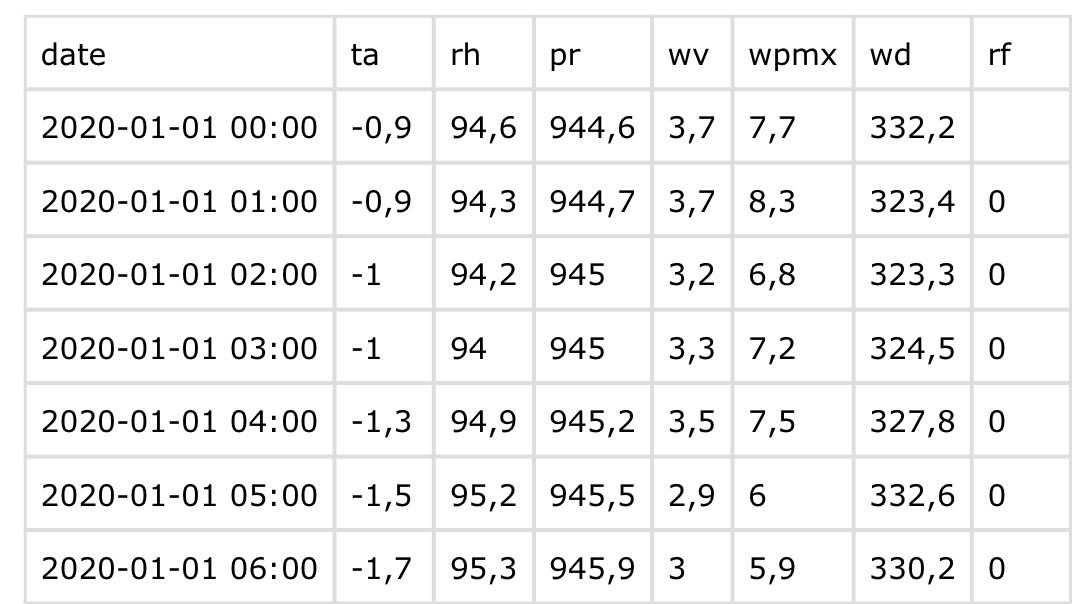
\includegraphics[scale=0.4]{Image.jpg}
	\caption{Dane meteorologiczne z Brennej}
	\label{fig:my_label}
\end{figure}

\section{Pierwsze Etapy Pipeline'u ML}
\subsection*{Cel wykorzystania danych}
Dane meteorologiczne mogą być wykorzystane w uczeniu maszynowym do różnych celów, takich jak: prognozowanie warunków pogodowych, klasyfikacja zdarzeń pogodowych, czy też dokładana predykcja wartości ciągłych, np. temperatury lub ilości opadów w mm. W tych przypadkach będziemy mówić o uczeniu nadzorowanym, ponieważ proces ten polega na wykorzystaniu danych wejściowych oraz odpowiednich etykiet, które model ma za zadanie przewidzieć.
\subsection{Inżynieria cech (FE), Eskploracja danych (EDA)}
\subsection*{Wartości brakujące}
\begin{figure}[h]
	\centering
	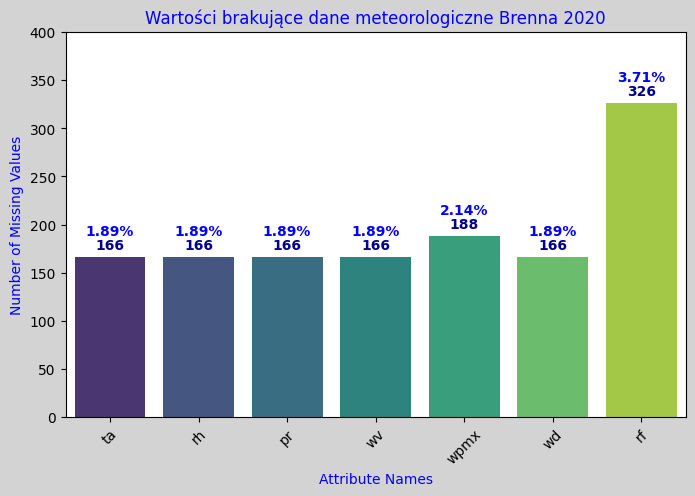
\includegraphics[scale=0.7]{ms_val.png}
	\caption{Wartości brakujące w danych meteorologicznych}
	\label{fig:my_label}
\end{figure}
\noindent W przypadku zmiennych takich jak ta, rh, pr, wv, wpmx, wd, liczba brakujących danych wynosi 166, co stanowi niewielki procent w porównaniu do całkowitej liczby próbek. Dla zmiennej rf (opady) brakujących wartości jest 326, co również jest małym procentem w odniesieniu do całkowitej liczby danych. W związku z tym, brakujące dane są stosunkowo niewielkie i nie mają istotnego wpływu na całościową strukturę danych.
\par
\hspace{0.75cm}
Biorąc pod uwagę niewielki procent brakujących danych oraz fakt, że braki są rozłożone równomiernie, można przyjąć, że brakujące wartości w danych meteorologicznych mają charakter Missing Completely at Random (MCAR). Oznacza to, że brakujące dane są losowe i nie zależą od innych zmiennych w zbiorze danych. Prawdopodobnie przyczyną braków odczytów były zakłócenia w pracy czujników lub inne techniczne problemy związane z urządzeniami pomiarowymi.
\par
\hspace{0.75cm}
W celu przygotowania danych meteorologicznych do modelowania zastosowano różne metody uzupełniania brakujących wartości, odpowiednio do charakteru poszczególnych zmiennych. Dla zmiennych ciągłych takich jak temperatura powietrza (ta), wilgotność względna (rh), ciśnienie atmosferyczne (pr), prędkość wiatru (wv), maksymalna prędkość porywu wiatru (wpmx) oraz kierunek wiatru (wd) zdecydowano się na interpolację liniową w funkcji czasu. Metoda ta pozwala na płynne oszacowanie brakujących wartości na podstawie danych sąsiednich, co odzwierciedla naturalne zmiany tych parametrów w czasie i zapewnia spójność czasową pomiarów.
\par
\hspace{0.75cm}
W przypadku zmiennej dotyczącej opadów (rf) przyjęto inne podejście: brakujące wartości zostały zastąpione zerami. Należy podkreślić, że w kolumnie rf występują zarówno wartości zerowe, jak i liczbowe (np. 0.2 mm, 4.2 mm), wskazujące ilość zmierzonego opadu. Jednak ze względu na charakter dalszej analizy, która będzie koncentrować się na określeniu samego faktu wystąpienia opadu (tak/nie), a nie na przewidywaniu dokładnej jego ilości, taka metoda imputacji została uznana za uzasadnioną. Nawet jeśli w godzinowych danych pojawią się pewne braki uzupełnione zerami, to ich wpływ na decyzję o klasyfikacji dnia jako deszczowego lub bezdeszczowego będzie pomijalny. Kluczowe jest zachowanie informacji o faktycznym wystąpieniu deszczu, natomiast pojedyncze uzupełnienia zerami w miejscach braku danych nie wprowadzą istotnych błędów analitycznych.

\subsection*{Kardynalność cech}
\begin{figure}[h]
	\centering
	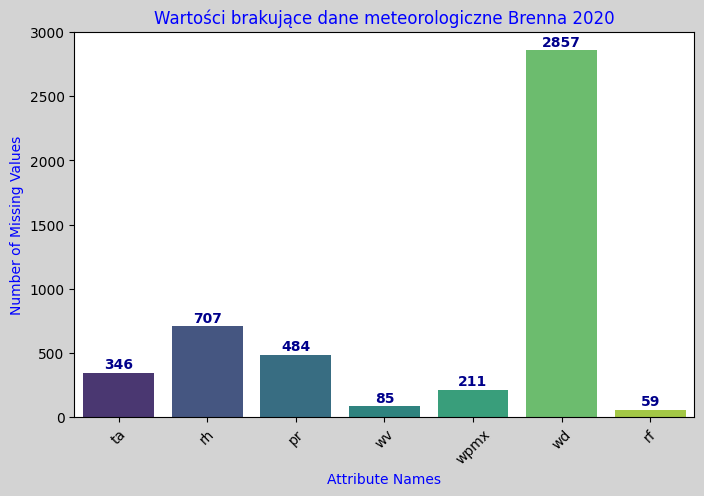
\includegraphics[scale=0.7]{cardinality.png}
	\caption{Kardynalność cech}
	\label{fig:my_label}
\end{figure}
\noindent W przedstawionych wynikach liczby unikalnych etykiet zmiennych, zauważalna jest szczególnie wysoka kardynalność w przypadku zmiennej wd (kierunek wiatru), która liczy aż 2857 unikalnych wartości. Taki wynik jest wynikiem precyzyjnego pomiaru w stopniach, co skutkuje dużą liczbą unikalnych kategorii. Pozostałe zmienne, takie jak temperatura (ta), wilgotność (rh), ciśnienie (pr), prędkość wiatru (wv), maksymalna prędkość porywu wiatru (wpmx) oraz opady (rf), wykazują raczej umiarkowaną liczbę unikalnych wartości, co jest typowe dla danych meteorologicznych i nie stanowi problemu w dalszej analizie.
\par
\hspace{0.75cm}
W celu uproszczenia analizy danych meteorologicznych, zdecydowano się na redukcję niektórych zmiennych. W przypadku zmiennej wd (kierunek wiatru), która posiada dużą liczbę unikalnych wartości, wprowadzono kategoryzację na osiem głównych kierunków: Północ, Północny Wschód, Wschód, Południowy Wschód, Południe, Południowy Zachód, Zachód i Północny Zachód. Takie podejście pozwala na zachowanie większej precyzji w analizie, jednocześnie zmniejszając liczbę unikalnych etykiet, co upraszcza modelowanie bez utraty istotnych informacji o kierunku wiatru.
Dla zmiennej rf (opady), zmiana jej na wartość binarną (0 – brak opadów, 1 – opady wystąpiły) została uznana za odpowiednią. Dzięki temu, zamiast analizować dokładną ilość opadów, skupiono się na wykrywaniu samego faktu wystąpienia opadów, co upraszcza modelowanie, szczególnie w przypadku klasyfikacji.
Pozostałe zmienne, takie jak temperatura, wilgotność czy ciśnienie, pozostają w oryginalnej formie, ponieważ zawierają cenne informacje, które mogą wpływać na przewidywania związane z opadami i innymi zjawiskami meteorologicznymi.

\subsection*{Wartości odstające}
\begin{figure}[h]
	\centering
	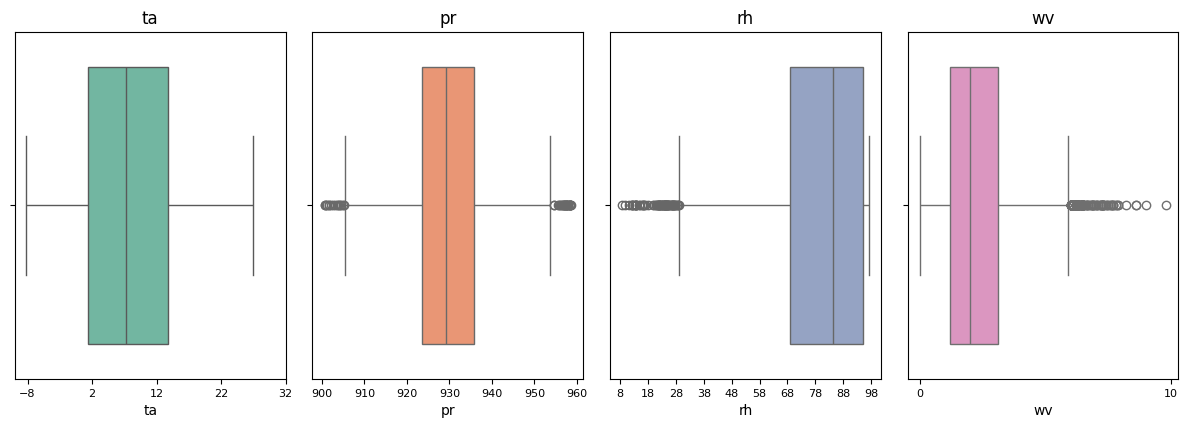
\includegraphics[scale=0.5]{boxplot.png}
	\caption{Wartości odstające}
	\label{fig:my_label}
\end{figure}
\noindent Po przeprowadzeniu analizy danych w celu odnalezniie anomalii nie wykryto obecności wyraźnych wartości odstających (outlierów) w zestawie danych meteorologicznych. Wszystkie zmienne rozkładają się w sposób typowy dla danych tego typu, a wartości skrajne, jeśli występują, nie odbiegają znacząco od ogólnych wzorców. W związku z tym, dane zostały uznane za stabilne i nie wymagały dalszej obróbki w zakresie usuwania wartości odstających.

\newpage

\subsection{Uczenie nadzorowane}
\subsection*{Przygotowanie danych pod uczenie nadzorowane}
\begin{figure}[h]
	\centering
	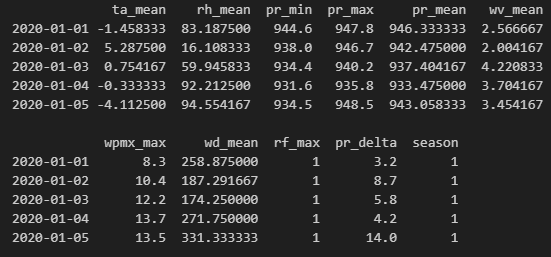
\includegraphics[scale=1]{df_prepare.png}
	\caption{Tabela danych przeprocesowanych}
	\label{fig:my_label}
\end{figure}
\noindent W celu przygotowania danych do uczenia nadzorowanego, ograniczono zbiór danych z poziomu godzinowego do dziennego. Zabieg ten miał na celu uproszczenie struktury danych oraz umożliwienie lepszego wykrywania powiązań między zmiennymi. Dodatkowo, wprowadzono nowe kolumny takie jak: pr\_min, pr\_max, pr\_delta (różnica między maksymalnym a minimalnym ciśnieniem w ciągu dnia) oraz season (pora roku: wiosna, lato, jesień, zima), aby wzbogacić zbiór o zmienne potencjalnie istotne dla procesu uczenia. Dla większości zmiennych obliczono średnią dzienną (mean), natomiast dla prędkości porywu wiatru (wpmx) zachowano wartość maksymalną w ciągu dnia, aby nie tracić informacji o ekstremalnych zjawiskach.

\subsection*{Wybór zmiennej Target}
\noindent Jako zmienną TARGET do uczenia nadzorowanego wybrałem zmienną rf (rainfall – opady). Wybór ten uzasadniam tym, że opady atmosferyczne są zjawiskiem istotnym meteorologicznie, a ich przewidywanie ma duże znaczenie praktyczne (np. w rolnictwie, transporcie czy zarządzaniu ryzykiem pogodowym). Ponadto zmienna rf dobrze nadaje się do klasyfikacji binarnej ("czy wystąpił opad: tak/nie"), co upraszcza zadanie predykcyjne i jest odpowiednie do zastosowania różnych algorytmów uczenia nadzorowanego.

\subsection*{Wybór zmiennych Features}
\noindent W celu wyznaczenia zmiennej TARGET (rf – opady deszczu) wybrałem podzbiór zmiennych FEATURES: pr\_min, pr\_max, pr\_delta, ta, rh oraz season Wybór tych cech został dokonany na podstawie wiedzy dziedzinowej o procesach meteorologicznych bez wykorzystywania algorytmicznych technik selekcji ważności zmiennych pr\_min, pr\_max oraz pr\_delta (minimalne, maksymalne ciśnienie i zmiana ciśnienia) zostały wybrane, ponieważ ciśnienie atmosferyczne jest kluczowym wskaźnikiem zmieniających się warunków pogodowych Nagłe spadki ciśnienia często zwiastują pogorszenie pogody i występowanie opadów dlatego wartości minimalne, maksymalne oraz zmiana ciśnienia w ciągu dnia mogą mieć istotny wpływ na predykcję opadów ta (średnia temperatura powietrza) została wybrana ponieważ temperatura wpływa na możliwość kondensacji pary wodnej w atmosferze Wyższe temperatury sprzyjają parowaniu, natomiast spadki temperatury mogą prowadzić do powstawania opadów rh (średnia wilgotność względna) również została uwzględniona gdyż wilgotność powietrza bezpośrednio wpływa na procesy tworzenia chmur i opadów season (pora roku) pozwala uwzględnić sezonowość występowania opadów, gdyż w różnych porach roku warunki atmosferyczne sprzyjające deszczowi mogą się znacząco różnić dlatego dodanie tej zmiennej umożliwia lepsze odwzorowanie zmienności w danych meteorologicznych Podsumowując, wybrane zmienne uwzględniają zarówno czynniki fizyczne jak ciśnienie temperatura i wilgotność, jak i sezonowe zmienności pogodowe co może pozytywnie wpłynąć na skuteczność modelu predykcyjnego

\end{document}
